\documentclass[journal]{IEEEtran}

\usepackage[utf8]{inputenc}
\usepackage{cite}
\usepackage{amsmath,amssymb,amsfonts}
\usepackage{graphicx}
\usepackage{textcomp}
\usepackage{xcolor}
\usepackage{stfloats}
\usepackage{booktabs}
\usepackage{tabularx}
\usepackage{microtype}
\usepackage{balance}
\usepackage[hidelinks]{hyperref}

\ifdefined\pdfcompresslevel
\pdfcompresslevel=9
\fi
\ifdefined\pdfimageresolution
\pdfimageresolution=600
\fi

\def\BibTeX{{\rm B\kern-.05em{\sc i\kern-.025em b}\kern-.08em
 T\kern-.1667em\lower.7ex\hbox{E}\kern-.125emX}}

\begin{document}

\title{Genuine Price Anomaly Detection for Battery Storage Arbitrage: Recurrent Autoencoders, Q-Learning Dispatch, and Adversarial Robustness on Real Wholesale Market Data}

\author{Keshav~Aggarwal%
\thanks{}%
}

\maketitle

\begin{abstract}
The battery energy storage system (BESS) generates most of its profits from a few price spikes each year. It is important to detect these price spikes in order to generate profits through arbitrage. Previous studies have used price histories that contain artificially added spikes, treating them as corrupted data. In contrast, in reality, they should be viewed as indicators of profitability in wholesale energy arbitrage in day-ahead locational marginal price (LMP) markets. We use Long Short-Term Memory (LSTM) and Gated Recurrent Unit (GRU) autoencoders without supervision to find profitable price events from the unaltered data. The signal is used to create a Q-learning policy for tabular arbitrage, followed by an adversarial price-manipulation test of the system, with an added detection mechanism for the attack. The most significant innovation is the creation of a new analysis method based on the original (non-manipulated) price data and a seasonal rolling window. The difference here is that our work does not utilize the synthetic anomaly technique used in the earlier study. Our model is tested against 3 years (2023–2025) of raw day-ahead California ISO prices. The GRU autoencoder is more efficient than the LSTM one, providing an area under the receiver operating characteristic curve (AUROC) of 0.882 (0.894 for seasonal AUROC) and learning 25\% faster. The resultant signal leads to quadrupling Q-learning arbitrage gains and amounts to $\$11,957$ in the six months. In addition, our classifier achieves 89.1\% precision and 97.2\% AUROC, thereby minimizing financial costs related to attacks by 67.2\% and outperforming the economic precision requirement of $p^* = 33.4\%$. By comparison, the standard procedure demands an unrealistic level of accuracy of $p^* > 100\%$. It demonstrates a causally sound and actionable alternative to the synthetic-anomaly method of BESS benchmarking. It highlights the importance of testing anomaly-detection algorithms on actual settlements rather than artificially generated spikes.
\end{abstract}


\begin{IEEEkeywords}
Adversarial robustness, anomaly detection, battery energy storage systems (BESS), California Independent System Operator (CAISO), energy arbitrage, graph neural networks, reinforcement learning, time-series forecasting.
\end{IEEEkeywords}

\section{Introduction}
\label{sec:intro}

Electricity prices in California have grown considerably more unpredictable in recent years. Solar output during the afternoon sun usually pushes locational marginal prices (LMPs) down toward zero, and sometimes below it, only for prices to snap back once the sun sets and gas and coal plants jack up prices to cover the evening peak. BESS exploits this daily rhythm, charging their systems while power is cheap and discharging as prices climb.

Most days, these swings follow a pattern dictated by the work schedule and the weather. However, a battery's annual profits tend to depend on a handful of extreme hours. Hourly prices can soar over \$1,000/MWh during heatwaves, transmission outages, and sudden generator trips, and a 10 MW/10 MWh battery that discharges just once during such a spike can earn about as much as it would have made in a whole week otherwise. It is therefore a high priority for storage operators to detect these rare hours as soon as possible or to anticipate them. 

Past state-of-the-art (SOTA) approaches to anomaly detection in pricing have addressed the problem primarily from a cybersecurity perspective~\cite{Vulnerability_Analysis, AE_Anomaly, Xie_FDI, Kosut_Market_FDI, Liu_FDI_Power}. Such an approach starts from using historical data without anomalies, creates artificial price spikes, and checks if such anomalies are detected. Such an approach may be useful in defending against a cyber-attack. However, it cannot prove the actual trading process, the origins of prices, or the legal procedures governing market settlements. If a legitimate \$1,000/MWh price-spike anomaly is detected and battery discharge is disabled, an operator will incur significant losses.

Such a gap explains why, in the main experimental sections~\ref{sec:dataset}-\ref{sec:economics}, we use only the actual market prices, obtaining settlement information from California Independent System Operator's Open Access Same-Time Information System (CAISO's OASIS)~\cite{CAISO} website without any synthetic additions. In Section~\ref{sec:adversarial}, we investigate the second question, which arises together with the problem stated above: Does the attacker really inject fake spikes into this data flow?

Using historical market data has two pragmatic issues. The first is that the historical prices provided by market operators cannot be taken as ground-truth labels; therefore, the model needs to be validated for statistical consistency and, ultimately, profitability. The second and even more important issue is that mistakes are not symmetrical in any sense. While a mistake in image or text recognition is just an annoyance, a mistake that prevents the battery from discharging into a real \$1,000/MWh spike costs money.

The reasons behind these two problems, lack of labeled data and imbalanced misclassification costs, inspire the design choices made in this paper. The paper is valuable in the following three aspects:

\begin{enumerate} 
\item First, we perform a benchmarking of seven different detector architectures, Isolation Forest, a Variational Autoencoder (VAE), a denoising diffusion model, single-node LSTM and GRU autoencoders, a multivariate LSTM, and a graph attention network—on 25,944 hours of actual CAISO data, across five random seeds and two disjoint test windows, in order to find out which one performs best in detecting price spikes versus everyday diurnal fluctuations.

\item On top of the detection signal obtained from these tests, we then apply rules-based, directional, and reinforcement learning-based dispatch policies to understand how different types of dispatchers exploit the signal generated by the detectors to make decisions that yield the best results. We prove that tabular Q-learning achieves maximum exploitation of the anomaly-detection signal, leading to nearly a fourfold increase in arbitrage profits.

\item Furthermore, the introduced detector can be targeted by price feed poisoning attacks. To assess the economic feasibility of defense from an asymmetric-risk perspective, we introduce the economic break-even point precision $p^*$ and prove that threshold-based defenses fail economically ($p^* = 1.017 > 100\%$). On the contrary, our approach reaches the break-even point at 89.1\% precision ($p^* = 0.334$), mitigating up to 67.2\% of the attack losses.

\end{enumerate}

\section{Literature Review}
\label{sec:related}

This work sits at the intersection of electricity price forecasting~\cite{Price_Forecasting, Weron_EPF, Lago_EPF_Benchmark}, unsupervised time-series anomaly detection~\cite{AE_Anomaly, LSTM_Anomaly, Audibert_USAD, Zhang_MSCRED, Kieu_RNN_Ensemble}, generative modeling~\cite{VAE, DDPM, Xu_Donut_VAE}, and battery dispatch optimization~\cite{MPC_BESS, BESS, RL_Dispatch, Shi_BESS_Coopt, He_CAISO_BESS}.

\textbf{Electricity Prices and Anomaly Detection:}
Rolling statistics, moving averages, and local z-scores were traditional approaches for detecting abnormal price levels. Although these were simple approaches to apply, they have limitations: they assume constant thresholds that do not change with the seasons; a threshold set in winter to accommodate low load levels will always result in alarms in summer.

The deep models learn the usual 24-hour price pattern directly from historical data; there are no predefined patterns in our models. The recurrent autoencoders (LSTM, GRU) transfer the sequence states forward through time and compress each daily path to a small-size bottleneck and detect the moments when the error of reconstruction becomes large~\cite{LSTM_Anomaly, GRU}. On the other hand, the variational autoencoders encode price windows into a continuous latent space~\cite{VAE, Xu_Donut_VAE}, and the denoising diffusion probabilistic models (DDPM) add Gaussian noise to the input and learn to un-noise this process \cite{DDPM}. Large price spikes are unusual and harder to un-noise, thus leading to large errors.

\textbf{Battery Dispatch and Trading.}
For storage scheduling, commonly used methods include model predictive control (MPC)~\cite{MPC_BESS}, linear programming, and dynamic programming~\cite{BESS, Shi_BESS_Coopt}, while reinforcement learning is increasingly seen as an alternative to these methods~\cite{RL_Dispatch, Chen_DRL_BESS, Singh_V2G}. One of the flaws frequently found in benchmarks reported in the literature is an implicit assumption of clairvoyance about tomorrow's prices; when the optimizer is aware of the prices in advance, then there is no need for anomaly detection at all. This problem is avoided by ensuring that every dispatch instance is performed in a purely causal manner.

\section{Methodology}
\subsection{Data and Chronological Partitioning}
\label{sec:dataset}

We have 3 years of hourly day-ahead LMPs from CAISO from January 1, 2023, to December 31, 2025. We collected price data from the three primary trading hubs, SP15 (south), NP15 (north), and ZP26 (central California), and four ancillary services (Regulation Up, Regulation Down, Spinning Reserves, and Non-Spinning Reserves) for a total of 25,944 hourly observations. The additional price streams serve as auxiliary contextual information for multi-channel anomaly detection, reflecting the overall tightness of operating reserves. At the same time, the economic trading calculations only evaluate day-ahead energy arbitrage. 

Price anomalies were registered during the above-mentioned time frame, which was SP15, reaching its highest point of \$1,143.78/MWh on August 17, 2023, due to heatwaves in the region, and its lowest point of -\$41.33/MWh on May 19, 2024, due to excessive energy generation.

\begin{figure*}[!t]
\centering

\includegraphics[width=0.96\textwidth]{architecture.png}
\caption{System architecture. The raw CAISO price data undergoes causal feature extraction before Stage 1, which consists of an iForest pre-filter, followed by Stage 2, which consists of deep autoencoders and multi-node models. The five-seed ensemble then guides the battery dispatching policy and the defense filter.}
\label{fig:architecture}
\end{figure*}

For a more realistic evaluation of our algorithm's effectiveness, we break down the time period into three periods without any overlap among them: the training period between January 12, 2023 and December 31, 2024 (17,272 hours, approximately 23.7 months), validation period between January 1 and June 30, 2025 (4,272 hours, 5.9 months – used only for threshold calibration), and testing period between July 1 and December 31, 2025 (4,400 hours, 6 months, evaluated once). We additionally evaluate a six-month out-of-sample seasonal test period between January 1 and June 30, 2025. In California wholesale markets, Day-Ahead Market (DAM) clearing occurs for all 24 hours of the subsequent operating day at 13:00 $D-1$. But BESS commercial traders must place their bids for energy deliveries without knowledge of the settled prices at 10:00 AM, but they have to roll their exposures to real-time imbalances on 15-minute and 5-minute basis. We test our models using only causal 24-hour rolling windows in order to eliminate the problem of foreseeing.

\begin{table}[!t]
\centering
\caption{Nomenclature and Parameter Settings}
\label{tab:nomenclature}
\footnotesize
\renewcommand{\arraystretch}{1.15}
\begin{tabularx}{\columnwidth}{lX}
\toprule
\textbf{Symbol} & \textbf{Description} \\
\midrule
$s_t$ & Anomaly score for the 24-h window ending at hour $t$ \\
$H$ & Window length ($H = 24$\,hours) \\
$x_{t,h}, \hat{x}_{t,h}$ & Normalized observed and reconstructed price at hour $h$ \\
$Q(s, a)$ & Action-value estimate for state $s$ and action $a$ \\
$\alpha, \gamma$ & Q-learning rate ($\alpha=0.15$) and discount factor ($\gamma=0.95$) \\
$r_t$ & Net arbitrage cash return at hour $t$ (\$) \\
$SOC_t$ & Battery energy level at hour $t$ ($0 \le SOC_t \le 10$\,MWh) \\
$C, P_{\max}$ & Rated energy capacity (10\,MWh) and power limit (10\,MW) \\
$e, dt$ & Round-trip cycle efficiency ($e=0.80$) and interval ($dt=1$\,h) \\
$c_{\text{fee}}, c_{\text{deg}}$ & Market fee (\$0.50/MWh) and cell degradation (\$2.50/MWh) \\
\bottomrule
\end{tabularx}
\end{table}

Since it is not possible to use ground-truth anomaly flags in historical settlement prices, a flag is made available for post hoc evaluation only for reference. The flag is considered an hour with a flag when the price is above 4 median absolute deviations (MAD) from the 30 days moving median or within the top/bottom 0.5\% of historical prices (which happens 517 times in 25,944 hours, or 2.0\%). None of the models is provided access to the flag throughout the entire training process. Sensitivity analyses reveal that rankings of model families based on their performances are invariant with respect to the thresholds (3.0 to 5.0 MAD).

\subsection{Detection Pipeline and Model Formulations}
\label{sec:detectors}

The detection pipeline (Fig.~\ref{fig:architecture}) uses a two-level filtering approach: Isolation Forest is used to isolate and remove easy-to-detect outliers, followed by analysis of the remaining possible hours using a deep-sequence model. Nomenclature is presented in Table~\ref{tab:nomenclature}.

Discrete-time state-of-charge (SOC) dynamics govern the physical operation of the battery energy storage system:

\begin{equation}
SOC_{t+1} = SOC_t + \left( \eta_{\text{ch}} P_t^{\text{ch}} - \frac{1}{\eta_{\text{dis}}} P_t^{\text{dis}} \right) \Delta t,
\label{eq:soc_dynamics}
\end{equation}

subject to operational power rating and storage capacity limits:
\begin{align}
0 \le P_t^{\text{ch}} \le P_{\max}, \quad 0 \le P_t^{\text{dis}} \le P_{\max}, \label{eq:p_limits} \\
0 \le SOC_t \le C, \label{eq:soc_limits}
\end{align}
where $P_t^{\text{ch}}$ and $P_t^{\text{dis}}$ denote charging and discharging power at hour $t$, respectively, with $P_{\max} = 10$\,MW, $C = 10$\,MWh, and $\Delta t = 1$\,h. Symmetric one-way conversion efficiencies satisfy $\eta_{\text{ch}} = \eta_{\text{dis}} = \sqrt{e} = \sqrt{0.80} \approx 0.894$, guaranteeing a round-trip cycle efficiency of $e = \eta_{\text{ch}}\eta_{\text{dis}} = 0.80$.

The Stage 1 Isolation Forest~\cite{IForest} considers nine historical-only causal features: (i) trailing 6-hour linear price slope $\Delta p / \Delta t$, (ii) non-reversion ratio $|p_t - p_{t-1}| / (|p_{t-1} - p_{t-2}| + \epsilon)$, (iii) 1-hour price difference $(p_t - p_{t-1})$, (iv) 3-hour price difference $(p_t - p_{t-3})$, (v) 24-hour trailing robust $z$-score $(p_t - \text{median}_{24}) / \text{MAD}_{24}$, (vi) 168-hour trailing $z$-score, (vii) 24-hour rolling volatility $\sigma_{24}$, and (viii--ix) cyclic diurnal harmonics $(\sin(2\pi h / 24), \cos(2\pi h / 24))$ for hour-of-day $h \in \{0, \dots, 23\}$.

Subsequently, the selected windows are passed through the deep sequential model that considers normalized 24-hour sliding price vectors and evaluates their anomaly score by means of mean squared reconstruction error:

\begin{equation}
s_t = \frac{1}{H}\sum_{h=1}^{H}\left(x_{t,h}-\hat{x}_{t,h}\right)^2.
\label{eq:score}
\end{equation}
Usually, the autoencoder successfully reconstructs the price graph for the particular day. However, when prices increase suddenly, the compressed representation is unable to encode the change, and $s_t$ increases sharply.

Three models have been implemented in total. VAE has been trained for 40 epochs with the Adam optimizer~\cite{Adam} ($\text{lr}=10^{-3}$, batch size=64). The VAE architecture consists of fully connected networks with 48 neurons, and the bottleneck is modeled as an 8-dimensional Gaussian distribution~\cite{VAE}. LSTM-AE and GRU-AE map the price sequence through 32 recurrent neurons to an 8-dimensional bottleneck.

The neural network is trained using the Adam optimization algorithm~\cite{Adam}, with a learning rate of $10^{-3}$, a batch size of 32, and 40 training epochs. The training uses the mean squared error loss function~\cite{LSTM_Anomaly, GRU}. In the GRU case, the input and forget gates are used, which makes training 25\% faster but does not affect temporal dependencies. The DDPM learns how to reverse the procedure of adding noise to the data on discrete schedules~\cite{DDPM}. The inference step involves corrupting the window samples at four noise levels ($t \in \{0.10, 0.25, 0.40, 0.60\}$) over 16 iterations and averaging the residuals.

To explore the influence of the regional transmission environment on predictability, we also feed SP15, NP15, and ZP26 as inputs to two multi-hub models, which include a 3-channel multivariate LSTM (MV-LSTM) control and a graph neural network autoencoder (GNN-AE)~\cite{GAT}. In the GNN-AE model, we use the graph representation $\mathcal{G} = (\mathcal{V}, \mathcal{E})$ for the three regional hubs, where $\mathcal{V} = \{\text{NP15}, \text{ZP26}, \text{SP15}\}$, and the edge set $\mathcal{E}$ contains the main transmission connections for Path 15 (between NP15 and ZP26) and Path 26 (between ZP26 and SP15). In the graph attention network, two graph attention layers are used (hidden units of 8), and the directional spatial attention weight $\alpha_{ij}$ is calculated as:

\begin{equation}
\alpha_{ij} = \frac{\exp\left(\text{LeakyReLU}\left(\mathbf{a}^T [\mathbf{W} h_i \parallel \mathbf{W} h_j]\right)\right)}{\sum_{k \in \mathcal{N}_i} \exp\left(\text{LeakyReLU}\left(\mathbf{a}^T [\mathbf{W} h_i \parallel \mathbf{W} h_k]\right)\right)},
\label{eq:gat}
\end{equation}

where $\mathbf{W} \in \mathbb{R}^{8 \times d}$ is a shared projection matrix, $\mathbf{a}$ is the attention vector, $\parallel$ is concatenation, and $\mathcal{N}_i$ denotes neighboring regional hubs. Spatial node representations are followed by LSTM-based temporal sequence encoding.

We conducted all experiments using five random seeds (0 to 4), ensuring that \texttt{torch.set\_num\_threads(1)} was always set and that cuDNN flags were fixed to ensure determinism.

\begin{table*}[!t]
\centering
\caption{Performance Master Summary: Accuracy of Model Reconstruction and Anomaly Identification}
\label{tab:detector_results}
\footnotesize
\renewcommand{\arraystretch}{1.2}
\setlength{\tabcolsep}{3.5pt}
\begin{tabular*}{\textwidth}{@{\extracolsep{\fill}}lccccccccc@{}}
\toprule
& \multicolumn{2}{c}{\textbf{Reconstruction Error ($\downarrow$)}} & \multicolumn{4}{c}{\textbf{Anomaly Detection Accuracy ($\uparrow$)}} & \multicolumn{3}{c}{\textbf{Operating Point Metrics ($\uparrow$)}} \\
\cmidrule(lr){2-3} \cmidrule(lr){4-7} \cmidrule(lr){8-10}
\textbf{Model Architecture} & \textbf{RMSE (\$)} & \textbf{MAE (\$)} & \shortstack{\textbf{Mean}\\\textbf{AUROC}} & \shortstack{\textbf{Ens.}\\\textbf{AUROC}} & \shortstack{\textbf{Avg.}\\\textbf{Prec.}} & \shortstack{\textbf{W2}\\\textbf{AUROC}} & \shortstack{$\boldsymbol{F_1}$\\\textbf{Score}} & \textbf{Precision} & \textbf{Recall} \\
\midrule
\multicolumn{10}{l}{\emph{Single-Node Models (Evaluated on CAISO SP15 Hub)}} \\
iForest & n/a & n/a & $0.623\pm0.030$ & 0.624 & 0.138 & 0.453 & $0.222\pm0.028$ & 0.227 & 0.217 \\
VAE & $7.85\pm0.47$ & $6.21\pm0.39$ & $0.534\pm0.164$ & 0.576 & 0.007 & 0.673 & $0.027\pm0.021$ & 0.015 & 0.226 \\
Diffusion (DDPM) & n/a$^\dagger$ & n/a$^\dagger$ & $0.564\pm0.071$ & 0.631 & 0.009 & 0.744 & $0.016\pm0.015$ & 0.009 & 0.096 \\
\textbf{LSTM-AE} & $10.37\pm1.76$ & $8.44\pm1.45$ & $\mathbf{0.738\pm0.145}$ & \textbf{0.859} & \textbf{0.184} & \textbf{0.921} & $0.107\pm0.099$ & 0.073 & 0.261 \\
\textbf{GRU-AE} & $9.70\pm0.68$ & $7.77\pm0.68$ & $0.776\pm0.237$ & 0.882 & 0.162 & 0.894 & $0.157\pm0.152$ & 0.110 & 0.304 \\
\midrule
\multicolumn{10}{l}{\emph{Multi-Node Spatial Models (Simultaneously Processing All 3 Regional Hubs: NP15, SP15, ZP26)}} \\
MV-LSTM Control & $9.12\pm0.84$ & $7.15\pm0.72$ & $0.854\pm0.165$ & 0.926 & 0.201 & n/a & $0.185\pm0.092$ & 0.142 & 0.326 \\
\textbf{GNN-AE} & $8.86\pm0.65$ & $6.94\pm0.58$ & $\mathbf{0.938\pm0.098}$ & \textbf{0.985} & \textbf{0.246} & n/a & $\mathbf{0.246\pm0.081}$ & 0.212 & 0.391 \\
\bottomrule
\end{tabular*}
\vspace{2pt}
{\raggedright \scriptsize \textbf{Notes:} $\downarrow$ Lower error is preferred; $\uparrow$ Higher accuracy is preferred. $^\dagger$Diffusion scores are derived from normalized noise residuals; iForest lacks a decoder. Multi-node setups process SP15, NP15, and ZP26 simultaneously.\par}
\end{table*}

\section{Detection Results and Model Comparison}
\label{sec:eval}

Thresholds for the budget percentile range from 0.5\% to 10\% were optimized based on the F1 score on the validation dataset and fixed prior to evaluating the model on the test dataset.

The results for the quality of reconstruction and detection of anomalies by all methods are provided in Table~\ref{tab:detector_results}, measured in terms of root mean squared error (RMSE) and mean absolute error (MAE). The receiver operating characteristic (ROC) curves are shown in Fig.~\ref{fig:roc}, while Fig.~\ref{fig:timeline} shows detection results compared with the SP15 market price.

\begin{figure}[!t]
\centering

\includegraphics[width=\columnwidth]{roc_curves.png}
\caption{Test-window receiver operating characteristic (ROC) curves for the 5-seed ensemble models on CAISO data, GRU-AE (downward triangle), LSTM-AE (diamond), Diffusion (upward triangle), iForest (circle), VAE (square), with the inset showing the operational low-false-positive region (false positive rate $\text{FPR} \le 0.12$).}
\label{fig:roc}
\end{figure}

Perhaps the most obvious trend from Table \ref{tab:detector_results} is that low reconstruction error does not necessarily indicate high-quality anomaly detection. While the VAE yielded the highest-quality reconstructions out of all single-node models (RMSE \$7.85/MWh), it generated the lowest detection scores (AUROC = 0.534; $F_1$ = 0.027). The VAE relies on the latent prior to generate Gaussian noise, so the output becomes smoothed, eliminating the exact signals needed for anomaly detection.

\begin{figure*}[!t]
\centering

\includegraphics[width=0.96\textwidth]{test_timeline.png}
\caption{Price spike identification for 6-month test data SP15 using reference (closed circles) and LSTM-AE (open squares) detection; it is clearly visible that the LSTM-AE detection agrees with the price spikes.}
\label{fig:timeline}
\end{figure*}

This is because recurrent autoencoders exhibited far better performance since they could handle temporal dependencies effectively. The AUROC values for the LSTM-AE and GRU-AE models were 0.859 and 0.882, respectively. As for the reason behind their superiority in this matter, one should note that, due to the sequential updating process, recurrent models maintain their memory of a typical daily pattern. Thus, upon encountering a sudden price change, the hidden state will be unable to reconcile the jump, and the error rate will skyrocket.

Incorporating price information from the three California centers increased the GNN-AE's mean AUROC to 0.938. However, the simple multivariate LSTM baseline performed nearly as well, achieving a mean AUROC of 0.854 and reaching 0.988 AUROC on three of the five seeds. Comparison of the two with a paired bootstrap yielded a 95\% confidence interval of $[-0.102, +0.281]$; as the interval includes zero, there is no statistically significant difference between using graph attention and using multivariate modeling alone. The added value seems to be mostly due to tracking price behavior in neighboring regions, rather than to graph attention.

The second test window for next year would demonstrate that the recurrent models can generalize across seasons, as the LSTM-AE achieved an AUROC of 0.921. On the other hand, the performance of the static Isolation Forest was extremely poor, as it could only get an AUROC of 0.453, worse than guessing randomly, because it is incapable of adapting to wholesale price variations from winter demand to summer solar/hydropower production.

The results obtained for a 5-channel diffusion model trained across all three hubs and two ancillary streams were an average AUROC of $0.528\pm0.066$, which is lower than the default at one hub ($0.564\pm0.071$). It seems like the additional price channels did nothing but add noise to the forward diffusion process, providing nothing to denoise on the reverse pass.

\subsection{Turning Detection into Profit}
\label{sec:economics}

To examine whether the anomaly alerts yield profits, we conducted trading simulations for a battery with a capacity of 10\, MWh/10\, MW ($e=0.80$, transaction cost \$0.50/MWh, degradation cost \$2.50/MWh~\cite{Xu_BESS_Degradation, Peterson_BESS_Degradation}).

Strategy 1 (Heuristic dispatch) is activated every time prices are less than the 25th percentile of the historical value and ends as soon as the prices become greater than the 75th percentile, with 5\, MW dispatch and 10\, MW dispatch as the event occurs. Strategy 2 (Directional spread) goes long or short 1\, MWh for every anomaly detected, with a 24-hour trading period. Strategy 3 (Tabular Q-learning)~\cite{Watkins_QLearning, Sutton_RL} learns to dispatch in a discrete state space defined by $s=(p_z, a_{\text{flag}}, s_{\text{soc}})$. Discrete z-normalized price is $N_p=10$ bins in the range from $-3$ to $+3$; anomaly flag is $N_a=5$ categories (or $N_a=1$ for unconditional version); battery state-of-charge ratio ($SOC_t/C$) is $N_s=5$ bins resulting in $|S|=250$ discrete states ($|S|=50$ without anomaly flag). The action space contains three discrete power actions $a \in \{-1.0, 0.0, 1.0\}$ corresponding to full discharge ($P_t^{\text{dis}}=P_{\max}$), idle ($P_t=0$), and full charge ($P_t^{\text{ch}}=P_{\max}$), subject to the physical constraints in \eqref{eq:soc_dynamics}--\eqref{eq:soc_limits}. The net cash return reward $r_t$ received by the agent accounts for market revenue, degradation, and fees:
\begin{align}
r_t ={}& \left( p_t P_t^{\text{dis}} - p_t P_t^{\text{ch}} \right) \Delta t \nonumber \\
&- \left[ c_{\text{fee}} \left( P_t^{\text{dis}} + P_t^{\text{ch}} \right) + c_{\text{deg}} P_t^{\text{dis}} \right] \Delta t.
\label{eq:reward}
\end{align}
The action values are iteratively learned in 30 training runs using Eq.~\eqref{eq:qlearning}:

\begin{equation}
Q(s,a) \leftarrow Q(s,a) + \alpha \left[r_t + \gamma \max_{a'} Q(s',a') - Q(s,a)\right],
\label{eq:qlearning}
\end{equation}
with learning rate $\alpha=0.15$, discount factor $\gamma=0.95$, and an $\epsilon$-greedy exploration schedule decaying linearly from $\epsilon_{\text{start}}=0.30$ to $\epsilon_{\text{end}}=0.02$.

\begin{table}[!t]
\centering
\caption{Arbitrage Earnings Across Both Test Windows (LSTM-AE Signal)}
\label{tab:economics}
\footnotesize
\renewcommand{\arraystretch}{1.15}
\setlength{\tabcolsep}{2.5pt}
\begin{tabularx}{\columnwidth}{Xcc}
\toprule
\textbf{Trading Strategy} & \textbf{Window 1 Profit} & \textbf{Window 2 Profit} \\
\midrule
Clairvoyant LP Upper Bound (Oracle) & \$16,840 & \$48,250 \\
Heuristic (Without / With Signal) & \$13,085 / \$13,089 & \$30,197 / \$30,762 \\
Directional Spread (Trades, Win\%) & \$487 (68, 76\%) & \$565 (84, n/a) \\
Q-Learning: Without Signal  & \$3,090 $\pm$ \$3,905 & \$23,451 $\pm$ \$3,180 \\
\textbf{Q-Learning: With Signal} & \textbf{\$11,957 $\pm$ \$393} & \textbf{\$35,567 $\pm$ \$3,658} \\
Deep Q-Network (DQN) (Without / With) & \$5,931 / \$5,246 & n/a \\
\bottomrule
\end{tabularx}
\end{table}

\begin{figure*}[!t]
\centering

\includegraphics[width=\textwidth]{profit_comparison.png}
\caption{Window 1 cumulative trading returns. (a) Heuristic dispatch, directional spread trading, and tabular Q-learning, showing how the anomaly signal nearly quadruples Q-learning profit while cutting seed variance tenfold. (b) Directional arbitrage profit and win rate across the four detector families.}
\label{fig:profit}
\end{figure*}

According to Table~\ref{tab:economics} and Fig.~\ref{fig:profit}, the profits from trading depend greatly on the degree of flexibility of the controller. To benchmark absolute policy efficiency, we evaluate the offline clairvoyant Linear Programming (LP) upper bound with perfect price foresight (at \$16,840 in Window 1 and \$48,250 in Window 2). Tabular Q-Learning without the anomaly signal is only able to reach 18.3\% of the oracle upper bound in Window 1; however, by adding the signal generated from the LSTM-AE model, the value becomes 71.0\% of the oracle upper bound (or 73.7\% in Window 2). In case of heuristic dispatching, the anomalous signal had almost no effect on profits (+0.03\% for Window 1, +1.87\% for Window 2) because power ratings and SoC constraints restrict the actions of static-threshold rules.

By contrast, directional spread trading revealed that the signal had value, as it delivered \$487 in profit with a 76\% success ratio, whereas under pure randomness it yielded only \$30.

The largest improvement was observed in Tabular Q-learning. The possibility for an agent to learn to use anomaly signals led to a near fourfold increase in Window 1 profit from \$3,090 to \$11,957 and a decrease in cross-seed standard deviation from \$3,905 to \$393 (-90\%). In addition, Window 2's profit increased by 51.7\% to \$35,567.

Nevertheless, Compute matched DQN~\cite{Mnih_DQN, Hasselt_DoubleDQN} gained \$5,246 profit using the signal, but the no-signal situation brought \$5,931 profit. Hence, continuous deep reinforcement learning was unable to handle reward noise in time series, whereas tabular Q-learning was able to generalize regardless of such noise. Please see Table~\ref{tab:perdetector} for the detailed results for each detector in Window 1, where LSTM-AE turned out to be the most efficient with 76\% win ratio and \$487 in spread profit.

\begin{table}[!t]
\centering
\caption{Per-Detector Arbitrage Performance (Window 1)}
\label{tab:perdetector}
\footnotesize
\renewcommand{\arraystretch}{1.12}
\setlength{\tabcolsep}{2.5pt}
\begin{tabular*}{\columnwidth}{@{\extracolsep{\fill}}lccc@{}}
\toprule
\textbf{Detector Family} & \textbf{Dispatch (\$)} & \textbf{Spread PnL (\$)} & \textbf{Trades, Win\%} \\
\midrule
iForest & \textbf{13,128} & 103 & 20, 68\% \\
VAE & 13,017 & 537 & 220, 61\% \\
Diffusion & 12,740 & 60 & 13, 77\% \\
\textbf{LSTM-AE} & 13,089 & \textbf{487} & \textbf{68, 76\%} \\
\bottomrule
\end{tabular*}
\end{table}

The VAE attains \$537 in spread profit from 220 transactions, as opposed to \$487 from 68 transactions in the LSTM-AE. On the other hand, the iForest attains the highest dispatch through the raw heuristic strategy (\$13,128). The model's high accuracy gives rise to the above contradiction. For example, the Gaussian latent bottleneck used by the VAE maintains persistently high reconstruction errors despite ordinary daily variations. It causes a very high number of transactions (220). However, it captures small intraday price variations by coincidence, with a low win rate (61\% versus 76\%), together with a much higher cost of cycling wear and transaction friction. However, the LSTM-AE initiates trades based on real price movements, achieving a very high win rate. Together with tabular Q-learning, which modulates the battery state-of-charge to anticipate the occurrence of a catastrophic event, the high-accuracy recurrent signal raises arbitrage profits fourfold.

\section{Adversarial Robustness: A Companion Study}
\label{sec:adversarial}

Another thing that we looked into was the reverse of the above problem, where the attacker would inject the price spikes into the feed system~\cite{Liang_FDI_StateEstimation, Kurt_FDI_Detection, Goodfellow_Adversarial}. In this case, the battery uses its stored energy and releases it during the price spike, making it appear to earn, but no money is made.

There were three kinds of attack profiles carried out for the SP15 price: Naive Multiplicative $3.0 \times$ attacks hourly; an 8-hour raised-cosine price attack intended to mimic the morning ramp attack profile; and multi-hour price wave attacks using sinusoidal prices. The defense mechanism uses the XGBoost predictor~\cite{XGBoost} based on 17 causal variables: z-score, trailing ratio, volatility, and consensus.

In Table~\ref{tab:adv_detect}, we see how much money is being lost without our defender: $-7.18\%$ for naive spikes, $-5.10\%$ for adaptive bumps, and $-15.11\%$ for sinusoidal waves. With our filter, we can recover the vast majority, 59.2\%, 36.5\%, and 67.2\%, of those losses, respectively, and come very close to our theoretical oracle bounds of 83.3\% to 94.0\%.

\begin{table}[!t]
\centering
\caption{Adversarial Detection and Economic Recovery (5 Seeds)}
\label{tab:adv_detect}
\scriptsize
\renewcommand{\arraystretch}{1.15}
\setlength{\tabcolsep}{0.6pt}
\begin{tabular*}{\columnwidth}{@{\extracolsep{\fill}}lcccc}
\toprule
\textbf{Attack} & \textbf{Recall} & \textbf{AUROC} & \textbf{Damage} & \textbf{Recovery (\%)} \\
\textbf{Profile} & & & \textbf{(\%)} & \textbf{($F_1$ / Cons. / Oracle)} \\
\midrule
Naive & $0.76\pm 0.07$ & $0.973\pm 0.026$ & $-7.18\pm 0.92$ & \textbf{59.2} / 33.8 / 89.1 \\
Adaptive & $0.66\pm 0.03$ & $0.971\pm 0.011$ & $-5.10\pm 0.89$ & \textbf{36.5} / 19.8 / 83.3 \\
Sinusoidal & $0.75\pm 0.02$ & $0.980\pm 0.011$ & $-15.11\pm 0.91$ & \textbf{67.2} / 66.2 / 94.0 \\
\bottomrule
\end{tabular*}
\end{table}

\subsection{Break-Even Precision Analysis ($p^*$)}

In the battery dispatch problem, a true positive (TP) identifies a fake spike, thus earning a profit ($v_{\text{TP}} > 0$). In contrast, a false positive (FP) misidentifies a genuine price spike, resulting in revenue loss ($v_{\text{FP}} < 0$). An operational defense that operates at a precision level of $p$ is said to be at the break-even point if the expected value of the cash flows:

\begin{equation}
p^* = \frac{v_{\text{FP}}}{v_{\text{FP}} - v_{\text{TP}}} = \frac{|v_{\text{FP}}|}{|v_{\text{FP}}| + v_{\text{TP}}}.
\label{eq:breakeven}
\end{equation}

\begin{table}[!t]
\centering
\caption{Break-Even Precision: Machine-Learning Classifier vs.\ Simple Threshold}
\label{tab:breakeven}
\footnotesize
\renewcommand{\arraystretch}{1.15}
\setlength{\tabcolsep}{2pt}
\begin{tabular*}{\columnwidth}{@{\extracolsep{\fill}}lcccc}
\toprule
\textbf{Defense Strategy} & \textbf{Prec.} & \shortstack{\textbf{\$/TP}\\\textbf{Saved}} & \shortstack{\textbf{\$/FP}\\\textbf{Lost}} & \shortstack{$\boldsymbol{p^*}$\\\textbf{Break-Even}} \\
\midrule
\textbf{Learned Classifier} & \textbf{0.891} & \$24.09 & $-\$19.11$ & \textbf{0.334} \\
Simple Robust-z Rule & 0.802 & $-\$4.89$ & $-\$350.45$ & \textbf{1.017} \\
\bottomrule
\end{tabular*}
\vspace{2pt}
{\raggedright \scriptsize \textbf{Notes:} Reported $p^*$ is the cross-seed/attack mean ($\mathbb{E}[p^*_i]$ across runs) rather than a ratio of aggregate column averages.\par}
\end{table}

\begin{figure*}[!t]
\centering
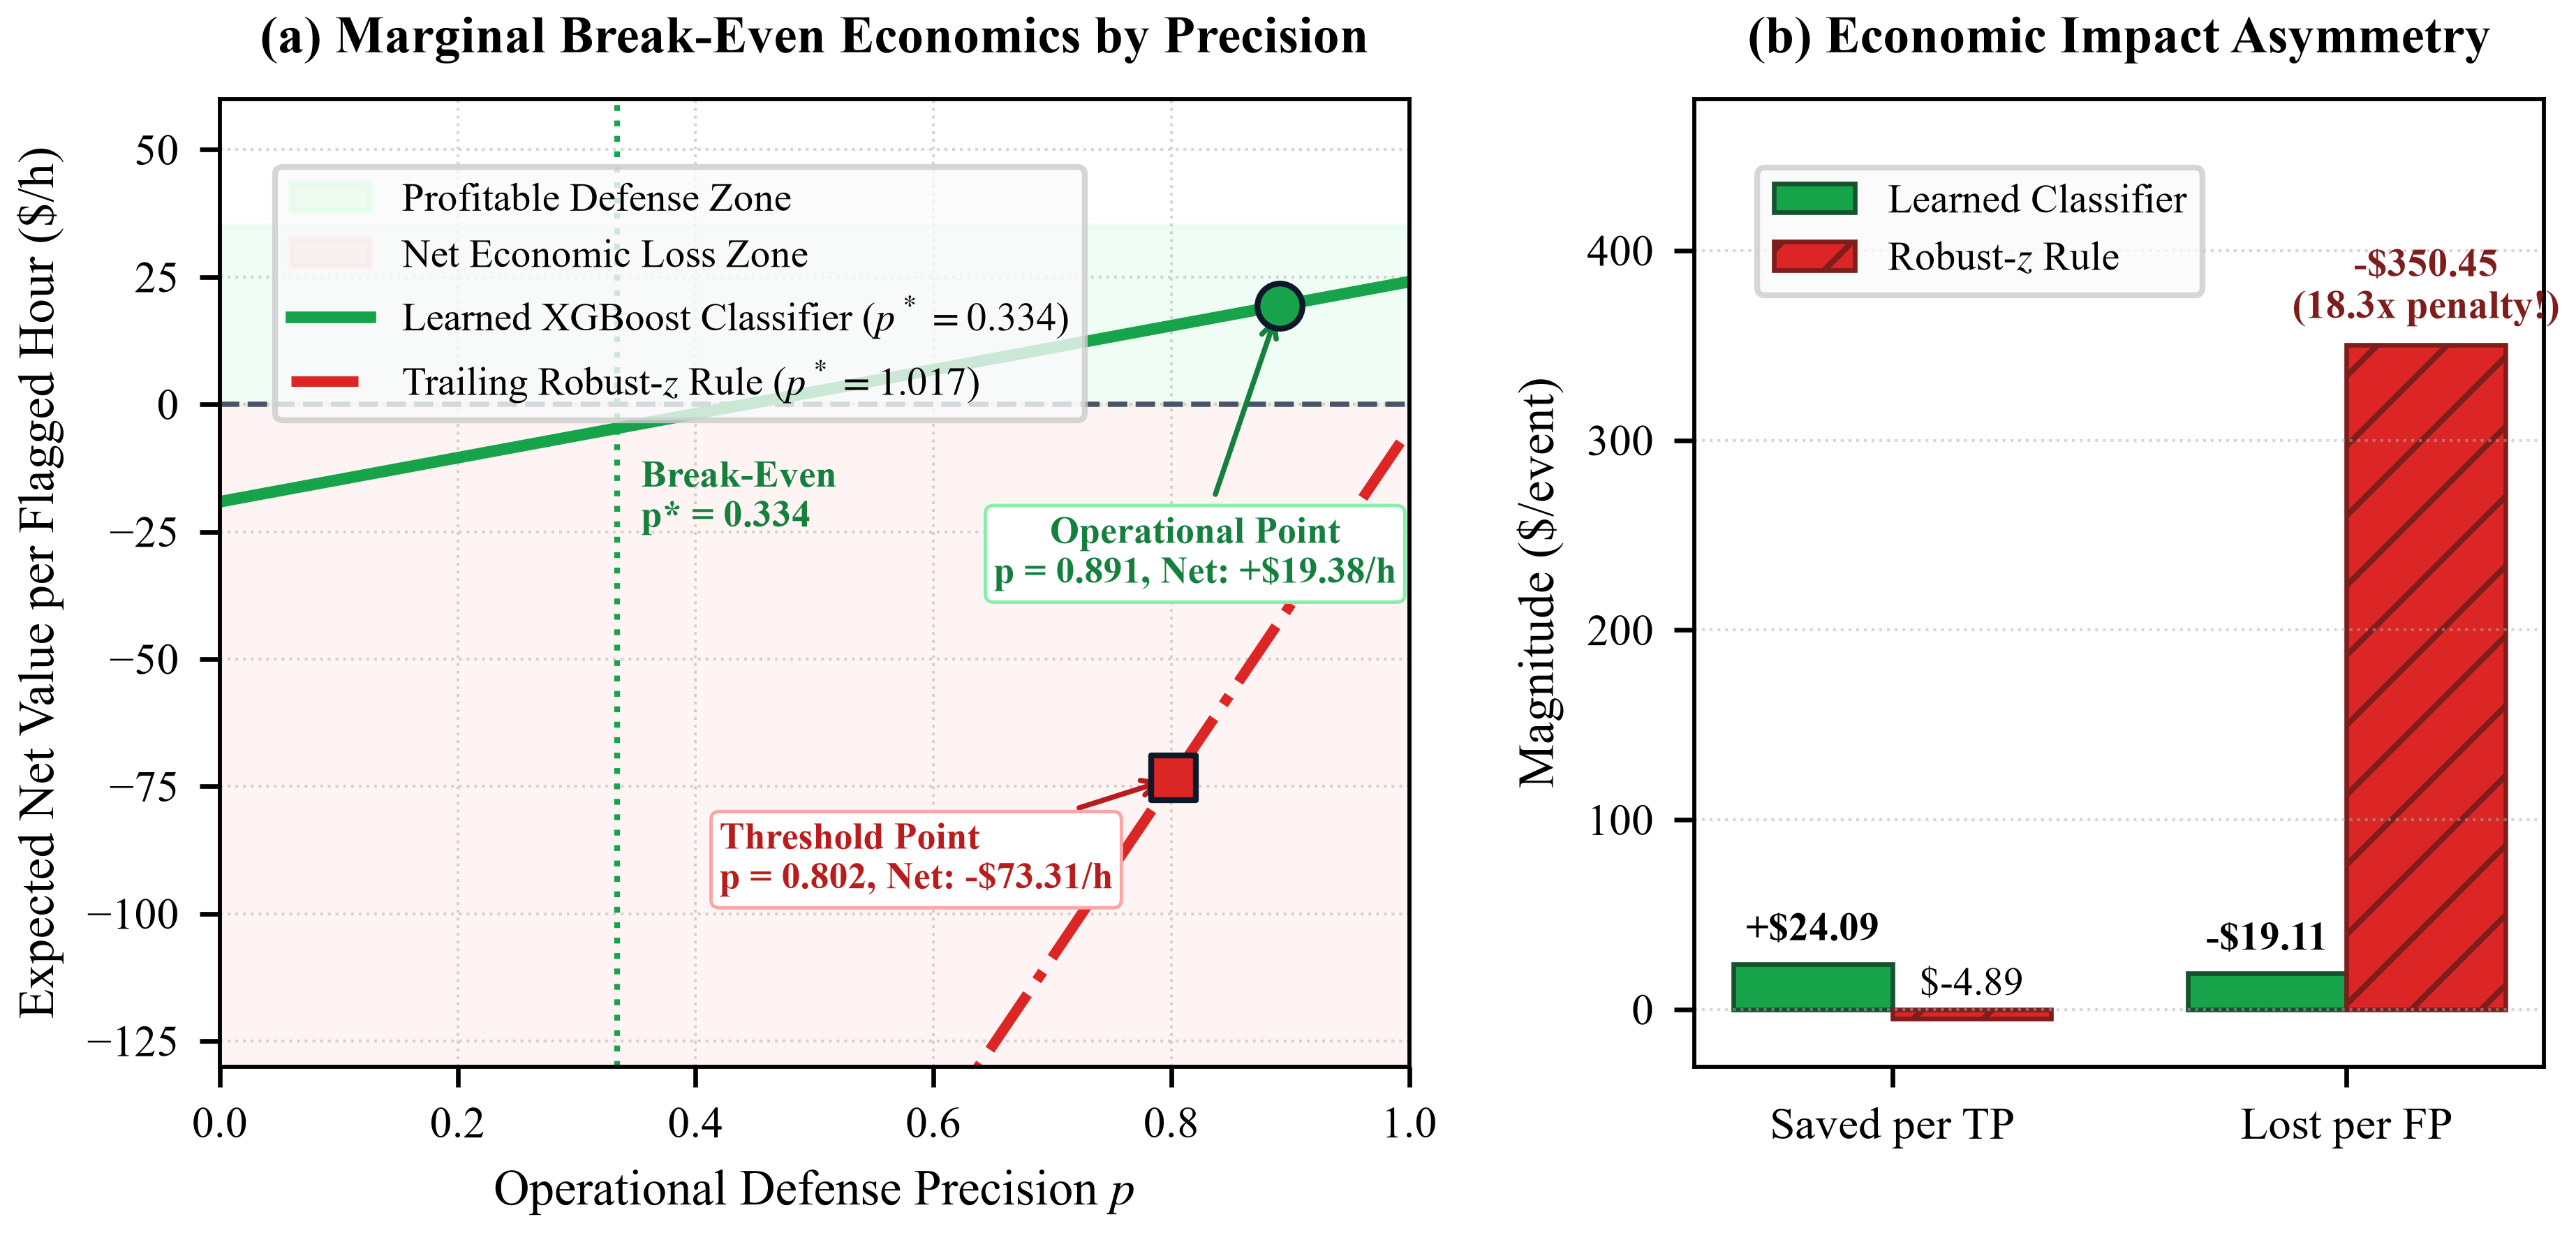
\includegraphics[width=\textwidth]{breakeven_tradeoff.png}
\caption{Break-even precision trade-off. (a) Net cash flow versus precision $p$ for the learned classifier ($p^*=0.334$, operating at $p=0.891$) against the simple threshold rule ($p^*=1.017$). (b) The asymmetry in false-alarm penalties: a threshold false alarm costs $18.3\times$ as much as a true positive saves.}
\label{fig:breakeven}
\end{figure*}

Economic differences between the learned classifier and the threshold-based classifier are quite remarkable (Table~\ref{tab:breakeven} and Fig.~\ref{fig:breakeven}). The learned classifier is estimated to save, on average, \$24.09 for every detected price spike and spend \$19.11 on each false alarm; hence, the break-even point is reached at the precision level of $p^* = 0.334$. Given that the learned classifier's actual precision is 89.1\%, it achieves robust economic surplus.

On the other hand, a robust-z threshold-based classifier is significantly less effective in terms of economic performance. This classifier incurs, on average, \$350.45 for each false alarm, approximately 18.3 times higher than for the learned classifier. Because high absolute values trigger the rule, it misses the year's most valuable price spikes; hence, its break-even point is $p^* = 1.017$, over 100\%.

\subsection{Generalization for Cross-Attacks}
From the cross-attacks experiments (Table~\ref{tab:transfer} and Figure~\ref{fig:transfer}), it becomes clear that defenders need to learn their defenses on different threat models. Nominal AUROC score stays above 0.75, while economic gain drops in the case when the threat model used in the attack is not known to the defender. For example, there was a decrease in economic gain by $40.9\%$ for a model that learned to defend from sinusoidal waves against adaptive bump attacks.

\begin{table*}[!t]
\centering
\caption{Cross-Attack Transfer Performance Across Source and Target Threat Types (5-Seed Average)}
\label{tab:transfer}
\footnotesize
\renewcommand{\arraystretch}{1.15}
\setlength{\tabcolsep}{8pt}
\begin{tabular}{llcccc}
\toprule
\textbf{Source Training Attack} & \textbf{Target Test Attack} & \textbf{AUROC} & \textbf{Precision} & \textbf{Recall} & \textbf{Recovery \%} \\
\midrule
Naive & Naive & 0.973 & 0.979 & 0.721 & 33.8 \\
Naive & Adaptive & 0.947 & 0.989 & 0.476 & $-18.0$ \\
Naive & Sinusoidal & 0.907 & 0.994 & 0.224 & 5.2 \\
Adaptive & Naive & 0.973 & 0.967 & 0.697 & 50.6 \\
Adaptive & Adaptive & 0.971 & 0.962 & 0.737 & 19.8 \\
Adaptive & Sinusoidal & 0.885 & 0.952 & 0.266 & 8.6 \\
Sinusoidal & Naive & 0.847 & 0.753 & 0.353 & 18.7 \\
Sinusoidal & Adaptive & 0.753 & 0.717 & 0.114 & $-40.9$ \\
Sinusoidal & Sinusoidal & 0.980 & 0.963 & 0.779 & 66.2 \\
\midrule
Adaptive + Sinusoidal & Naive & 0.960 & 0.881 & 0.674 & 43.2 \\
Naive + Sinusoidal & Adaptive & 0.937 & 0.995 & 0.352 & $-46.6$ \\
Naive + Adaptive & Sinusoidal & 0.902 & 1.000 & 0.200 & 3.9 \\
\bottomrule
\end{tabular}
\end{table*}

\begin{figure*}[!t]
\centering
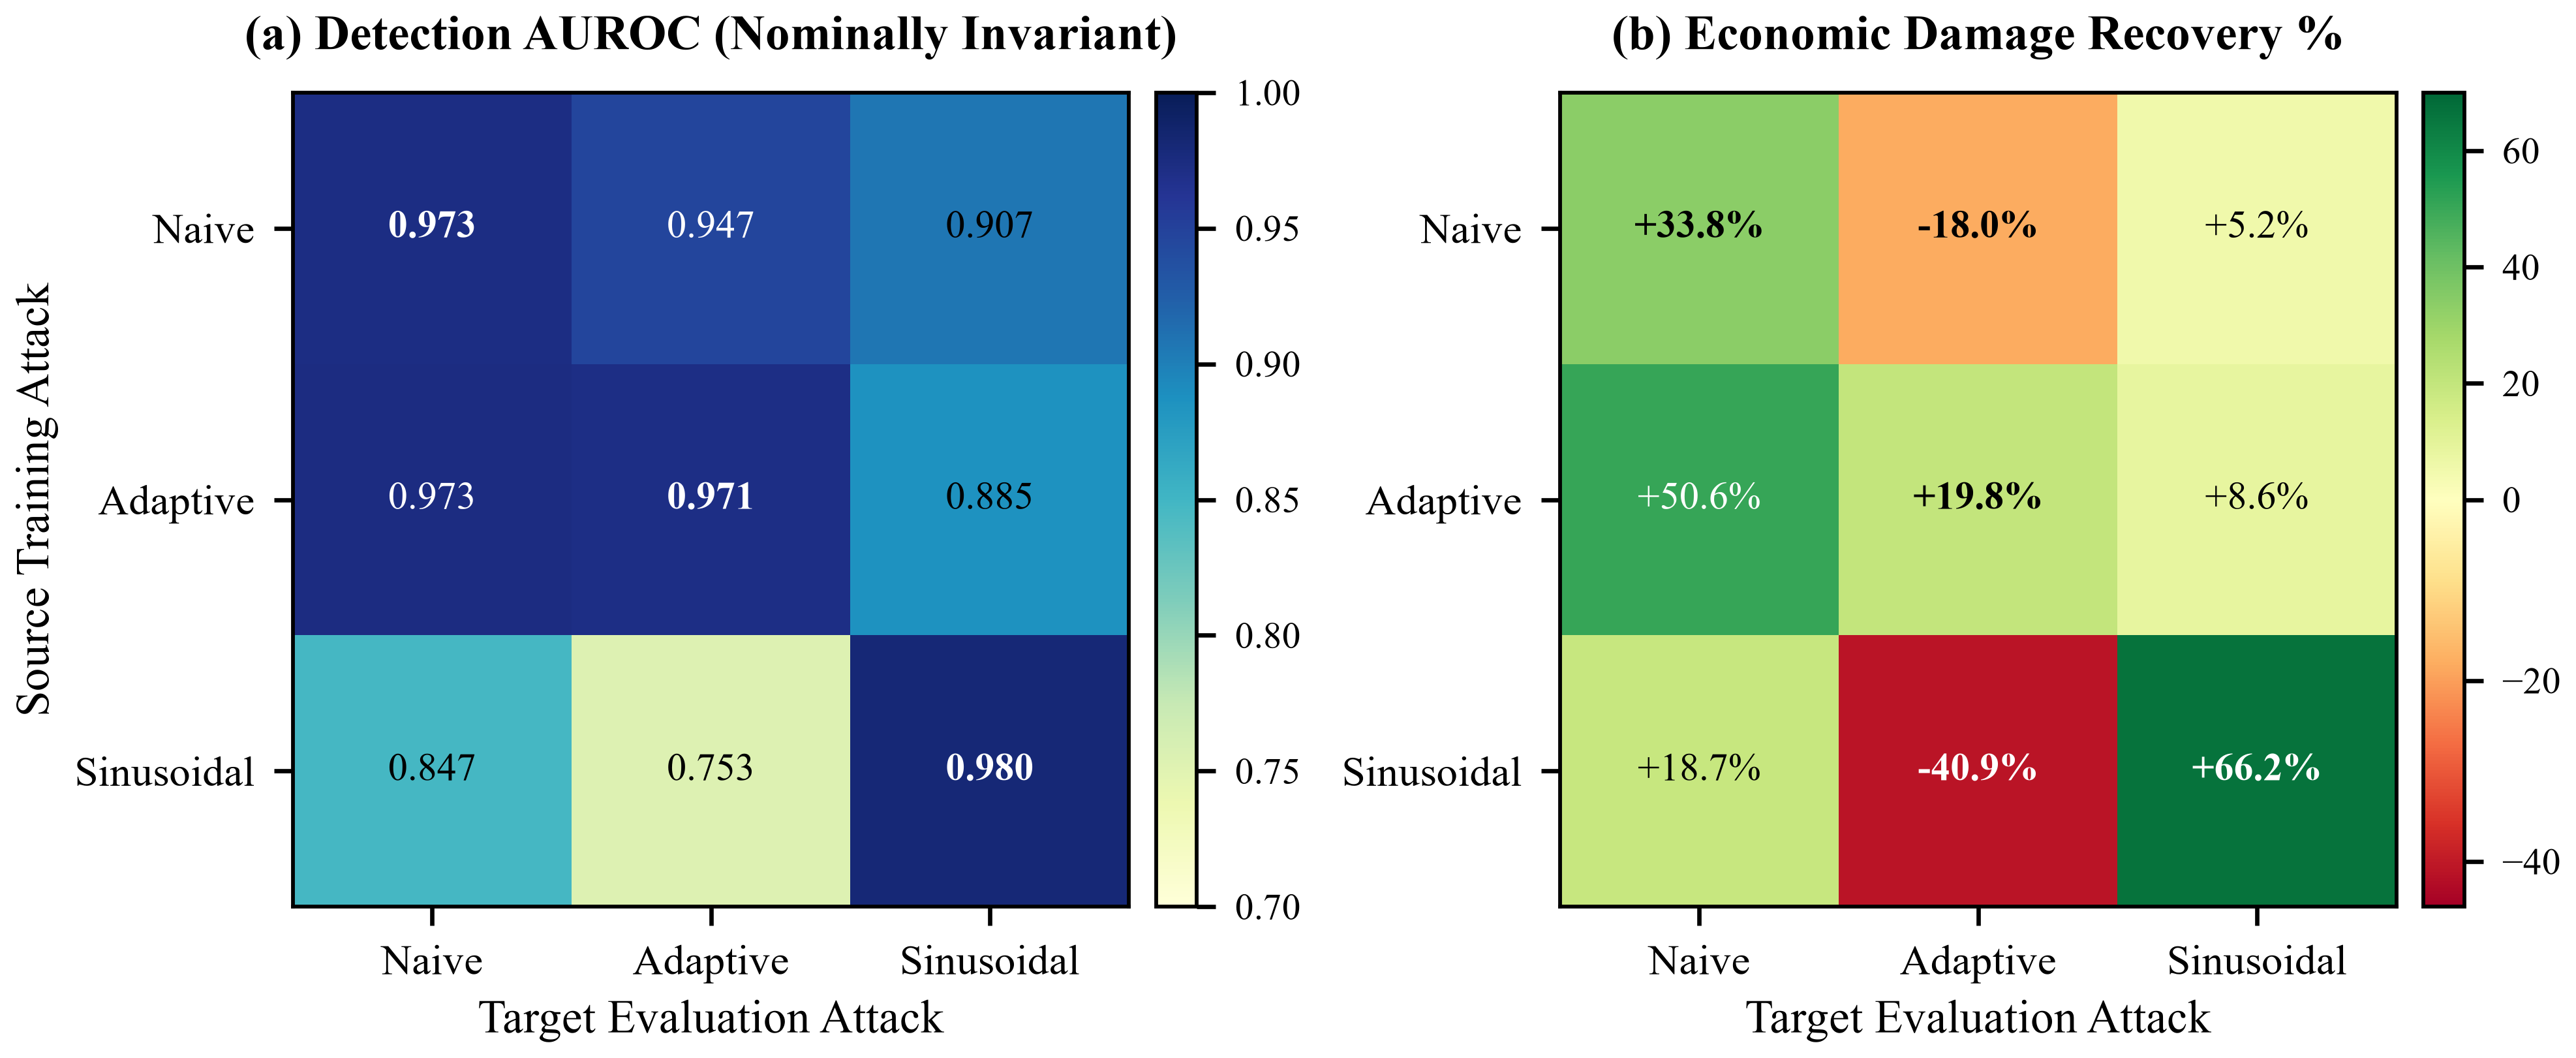
\includegraphics[width=0.96\textwidth]{transfer_heatmap.png}
\caption{Cross-attack transfer evaluation. (a) The detection AUROC Matrix shows that all values are very high ($\geq 0.75$). (b) Economic Recovery Matrix reveals serious cross-attack vulnerabilities; for example, a value of $-40.9\%$ between Sinusoidal and Adaptive attacks.}
\label{fig:transfer}
\end{figure*}

\section{Discussion, Limitations, and Future Work}
\subsection{Discussion and Practical Takeaways}
\label{sec:discussion}

The results can be applied in practice in three ways to storage in wholesale electricity markets.

Why do recurrent models emerge victorious in this case? Electricity prices are not independent samples from some distribution; they depend on the solar cycle, industrial activity, and the speed at which thermal power stations come online. Hence, when there is an unusual jump of \$800, an LSTM or GRU does not reconstruct this jump correctly because its internal state has been influenced by the previous 20 hours of normal diurnal dynamics, something which is impossible for a static model or a VAE, which treats all the hours equally.

Another clear implication is that anomaly-based solutions can work only when the defender has access to the alarm. Some algorithms would find it hard to apply the alarms because their deployment was based on the thresholds anyway. Tabular Q-learning, on the other hand, used this data to reduce energy usage during normal times and sell the saved energy at peak times.

The graphs definitely depict yet another important idea concerning securing the grid – that of being false positive on actual price spikes costing too much money. In order to compensate for losing \$350 due to a false positive just once, it is necessary to detect a few hundred successful attacks. Hence, a practical solution should first preserve the actual price spikes.

\subsection{Limitations and Future Work}
\label{sec:limitations}

The 4-MAD benchmark flag offers an objective, statistical standard for measuring detector discrimination; however, the ultimate standard is trade-off profitability. The cost of linear degradation in our simulation dispatches is estimated to be \$2.50 per MWh~\cite{Xu_BESS_Degradation, Peterson_BESS_Degradation}. The sensitivity analysis is conducted with reference to policy viability based on cell chemistry (for instance, Lithium Iron Phosphate [LFP] that suffers less degradation than Nickel Manganese Cobalt [NMC]), where we investigate the range of $c_{\text{deg}} \in [\$1.00, \$5.00]/\text{MWh}$ and $e \in [0.75, 0.90]$. Because wholesale market price spikes frequently reach \$200 to \$1,143/MWh, the gross spread margin overwhelmingly exceeds marginal cell aging costs during anomaly hours. Consequently, the optimal policy actions and the economic superiority of anomaly-informed dispatch remain invariant across realistic battery chemistries. Nevertheless, integrating non-linear cycle-depth rainflow counting with electrochemical cell thermal dynamics remains an important avenue for optimizing multi-year asset lifespans.

In our reinforcement learning experiments, we found that while tabular Q-learning is very robust, DQN-based approximations in continuous state spaces are prone to market disturbances and large reward variance. Although Day Ahead Market (DAM) data at an hourly resolution has helped us in providing a thorough and verifiable foundation for a three-year multi-hub analysis, its extension to Fifteen Minute Market (FMM) and Real-Time Dispatch (RTD) at a resolution of five minutes will enable storage systems operators to benefit from frequent sub-hour volatilities in the market. Finally, the multi-node analysis has been carried out for three major trading hubs of California.

\section{Conclusion}
\label{sec:conclusion}

This paper explored the problem of detecting price anomalies for BESS dispatch in wholesale electricity markets to make arbitrage more profitable and more resilient to adversarial conditions. The framework, combining deep recurrent autoencoders for anomaly detection and tabular Q-learning for the dispatch controller, was proposed, in which the autoencoder's output served as a signal for the controller's decision-making process and was tested under the strict causality assumption without data injection. With the use of 3 years of CAISO data on a day-ahead basis, it was observed that recurrent neural networks performed better than any other model used for single-hub anomaly detection, with GRU-AE (AUROC = 0.882) performing slightly better than LSTM-AE (AUROC = 0.859); and using this signal led to a Q-learning profit increase of \$8,867 (Window 1). Thus, it is evident that anomaly detection learning methods can offer greater efficiency not only in terms of accuracy but also economically compared with heuristic filters. The proposed method is ready to be implemented in the existing BESS system without any adjustments to the power market infrastructure, allowing operators to secure their income from BESS use. The dispatch controller will be extended to continuous state-action spaces using deep reinforcement learning and assessed for its transferability to other wholesale electricity markets and different grid topologies.

\bibliographystyle{IEEEtran}
\bibliography{references}

\end{document}